\subsection{Circle Packing}
\label{sec:circle-packing}


Circle packing considers arrangements of circles on surfaces
with the property that no two circles overlap. 
Dense packings are often desirable \cite{chang_simple_2010}.
In dense circle packings, all circles are touching other circles.
Given a circle packing one can construct the contact graph with a vertex for each
circle and an edge connecting tangent circles.

A disk triangulation graph is a graph $G=(V,E)$ that is planar, all interior faces
are triangles, the boundary of $G$ forms a simple closed polygonal chain, and each
vertex has finite degree (locally finite).  See \figref{circle-packing} for an example.
In \todo{find citation} proved the following remarkable theorem.

\begin{theorem}[Koebe-Andreev-Thurston (KAT)]\label{thm:kat}
Every finite, simple, planar graph can be represented as a circle packing in the plane.
\end{theorem}

\begin{figure}[htb]
        \centering
        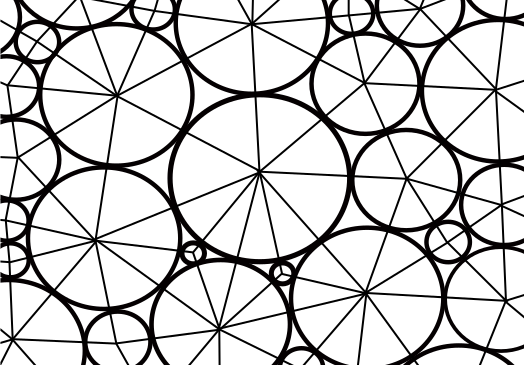
\includegraphics[width=.45\textwidth]{circle-packing}
		\caption{Part of an infinite circle packing and its corresponding contact graph.
		\label{fig:circle-packing}}
\end{figure}


Given disk triangulation graph the corresponding circle packing guaranteed
by \thmref{kat} assigns angles around all vertices in $V$.
Thus, for each vertex we can compute its discrete curvature given by
the circle packing,
$$K(v)=2\pi -\sum_{\text{angles at } v}\theta_i.$$
But this is our definition of discrete curvature!
The Gauss-Bonnet theorem holds using the circle packing metric on the vertices
of graphs which are used to model many important relationships.




\todo{gauss-bonnet all up in here\cite{gu_discrete_2013}}


Given an infinite disk triangulation graph $G$ with no information about
its circle packing, since $G$ is infinite, the corresponding circle packing either fills
the entire plane or it fills the unit disk.
The plane and the disk cannot be mapped bijectively to each other, thus
we can define the circle packing type. A disk triangulation graph $G$ is circle packing
 \emph{parabolic} if there exits a circle packing which fill the entire plane 
 whose contact graph is equivalent to $G,$ and $G$ is circle packing \emph{hyperbolic}
 if there exists a circle packing which fill the unit disk and whose contact graph
 is equivalent to $G$.

Suppose we are presented with a graph $G$ of disk triangulation with an infinite 
number of vertices, our task is to determine if $G$ is parabolic or hyperbolic
We next share an application of the Gauss-Bonnet theorem given by Oh in \cite{oh_criteria_2022},
to make this determination.






For each $n\in\NN$ let $B_n$ be the combinatorial ball of radius $n$
centered at a fixed vertex in $G.$ Let $k_n$ be the degree excess sequence
defined above, let $a_n=\sum_{j=0}^{n-1}(k_j+6)$ for $n=1,2,\ldots$.
Then $G$ is circle-packing parabolic if 

\begin{equation}\label{eqn:cp-parabolic}
\sum_{n=1}^{\infty}\frac{1}{a_n}=\infty,
\end{equation}

and $G$ is recurrent if

\begin{equation}\label{eqn:recurrent}
\sum_{n=1}^{\infty}\frac{1}{a_n+a_{n+1}}=\infty.
\end{equation}

As a consequence we have if

$$k_n=\sum_{v\in B_n}(\deg v -6)\leq c\ln n$$
for sufficiently large $n$, where $c$ is a fixed positive constant,
then $G$is circle-packing parabolic and recurrent.